\documentclass[a4paper,onecolumn,oneside,11pt,DIV=12]{scrartcl}

\usepackage[utf8]{inputenc}
\usepackage[english]{babel}
\usepackage{graphicx}
\usepackage{epsfig}
\usepackage{wrapfig}
\usepackage{float}
\usepackage{booktabs}
\usepackage{xspace}
\usepackage{color}
\usepackage{colortbl}
\usepackage[table]{xcolor}
\usepackage{attrib}
\usepackage{pgfgantt}
\usepackage{multirow,setspace}
\usepackage{footnote}
\usepackage[normalem]{ulem}
\usepackage{subcaption}
\usepackage{amsmath,amssymb}
\usepackage[inline]{enumitem}
\usepackage{url}

\usepackage{pgfgantt}
\usepackage[top=2cm, bottom=1.5cm, left=2cm, right=2cm]{geometry}

\usepackage{tikz}
\usetikzlibrary{shapes,arrows,positioning,backgrounds,fit,calc,shadows,decorations.pathreplacing,shapes.geometric, arrows.meta}

% Define colors
\definecolor{lightblue}{RGB}{225,245,254}
\definecolor{mediumblue}{RGB}{129,212,250}
\definecolor{lightgreen}{RGB}{232,245,233}
\definecolor{mediumgreen}{RGB}{165,214,167}
\definecolor{lightred}{RGB}{255,235,238}
\definecolor{mediumred}{RGB}{255,205,210}
\definecolor{lightorange}{RGB}{255,243,224}
\definecolor{mediumorange}{RGB}{255,204,128}
\definecolor{lightlime}{RGB}{241,248,233}
\definecolor{mediumlime}{RGB}{197,225,165}

% Orphan lines
\usepackage[all]{nowidow}

\newcommand{\aftersectionspacing}{2pt}
\newcommand{\beforesectionspacing}{.3}

\RedeclareSectionCommand[
  runin=false,
  afterindent=false,
  beforeskip=\beforesectionspacing\baselineskip,
  afterskip=\aftersectionspacing]{section}
  
\RedeclareSectionCommand[
  runin=false,
  afterindent=false,
  beforeskip=\beforesectionspacing\baselineskip,
  afterskip=\aftersectionspacing]{subsection}
  
\RedeclareSectionCommand[
  runin=false,
  afterindent=false,
  beforeskip=\beforesectionspacing\baselineskip,
  afterskip=\aftersectionspacing]{subsubsection}
  
\RedeclareSectionCommand[
  runin=false,
  afterindent=false,
  beforeskip=\beforesectionspacing\baselineskip,
  afterskip=\aftersectionspacing]{paragraph}

\usepackage{tikz,lmodern}
\usepackage[most]{tcolorbox}

\usepackage[acronym, nowarn]{glossaries}
\makeglossaries

\usepackage{tabularx}
\usepackage{longtable}
\raggedbottom
\newcommand{\tblsize}{\scriptsize}
\newcommand{\project}{FIND\xspace}

\usepackage[font=footnotesize,labelfont=bf,format=plain]{caption}

\usepackage{bibspacing}
\usepackage{csquotes}

% ============================================================
% ERC HEADER: PI last name — Acronym — Part B1/B2
% ============================================================
\usepackage{fancyhdr}
\pagestyle{fancy}
\fancyhf{}
\renewcommand{\headrulewidth}{0pt}
\fancyhead[L]{\small Lepperød}
\fancyhead[C]{\small FIND}
\fancyhead[R]{\small Part B1}
\fancyfoot[C]{\thepage}

% Command to switch to B2 header
\newcommand{\switchtobtwo}{%
  \fancyhead[R]{\small Part B2}%
}

% save bibliography space....
\usepackage{lmodern}
\usepackage[giveninits=true,backend=biber,doi=false,isbn=false,url=false,maxnames=5,sorting=none,style=numeric-comp]{biblatex}
\renewcommand{\bibfont}{\normalfont\normalsize}
\addbibresource{references.bib}
% Strip arXiv pseudo-DOIs (10.48550/*) so only eprint: is shown for preprints
\DeclareSourcemap{
  \maps[datatype=bibtex]{
    \map{
      \step[fieldsource=doi, match=\regexp{^10\.48550}, final]
      \step[fieldset=doi, null]
    }
  }
}
% Strip arXiv dblp field
\AtEveryBibitem{%
  \clearfield{dblp}%
}

\title{\vspace{-10mm}\Large{\project: Flexible Intelligence through Neurocomputational Design}}

%%%%%%%%%%%%%%%%%%%%%%%%%%%%
% TOGGLE CALL TEXT ON OR OFF
%%%%%%%%%%%%%%%%%%%%%%%%%%%%
%\newcommand{\calltext}[1]{\noindent\color{red}CALL-TEXT:\\ #1 \\ \color{black}}                 % DO include call text - ON
\newcommand{\calltext}[1]{}    % DO NOT include - OFF
%%%%%%%%%%%%%%%%%%%%%%%%%%%%

\date{}\author{} % show no date or author

\begin{document}

% ============================================================
% PART B1: Cover Page + Part I + CV/Track Record
% ============================================================
\begin{refsection}

% ============================================================
% ERC Starting Grant 2026 — Part B1 Cover Page
% ============================================================

\thispagestyle{empty}
\begin{center}
{\Large \textbf{ERC Starting Grant 2026}}\\[4mm]
{\Large \textbf{Part B1}}\\[8mm]

{\LARGE \textbf{Flexible Intelligence through Neurocomputational Design}}\\[4mm]

{\Large \textbf{\project}}\\[8mm]

\begin{tabular}{ll}
\textbf{Principal Investigator:} & Dr.\ Mikkel Elle Lepperød \\[2pt]
\textbf{Host Institution:} & Simula Research Laboratory, Norway \\[2pt]
\textbf{Duration:} & 60 months \\[2pt]
\textbf{Primary Panel:} & PE6 — Computer Science and Informatics \\[2pt]
\end{tabular}
\end{center}
\vspace{6mm}

\noindent\textbf{Abstract}

\noindent Current AI systems cannot selectively store and retrieve information across thousands of timesteps---a capability biological brains achieve routinely through distributed memory systems. Transformers forget beyond their context window; state space models compress everything into fixed-size state; and memory-augmented networks lack causal models to decide what is worth storing. FIND develops \textbf{PAM} (\textbf{P}redictive \textbf{A}ctive temporal coding with distributed \textbf{M}emory), a novel brain-inspired architecture where modules of neurons read and write to local long-term memory, combining temporal predictive coding, hyperdimensional computing, and active inference into a unified framework.

PAM combines three mechanisms: (1)~\textit{Distributed modular specialization} where each module maintains dedicated content-addressable memory; (2)~\textit{Temporal predictive coding} where prediction errors drive memory updates and learning; and (3)~\textit{Active inference} where action selection minimizes uncertainty. Our preliminary results demonstrate PAM's viability at scale: 100\% recognition accuracy on CORe50 (50 objects) with \textbf{zero catastrophic forgetting by construction}; \textbf{98.2\% online continual learning accuracy} across 120K samples in 55 seconds---12$\times$ faster than gradient-based methods; and \textbf{24.7\% exact match on ARC} (the Abstraction and Reasoning Corpus) with only 1.47M parameters, approximately 2$\times$ GPT-4o's 12\% at $>$1000$\times$ fewer parameters.

FIND will develop PAM through three work packages: \textbf{WP1} establishes temporal predictive coding with distributed memory for continual learning and long-range temporal reasoning; \textbf{WP2} extends this to compositional reasoning and program synthesis through neurosymbolic HDC integration; and \textbf{WP3} stress-tests the system in demanding open-ended environments (Memory Maze, Minecraft, Factorio) requiring planning and adaptation across $>$10,000 timesteps.

\newpage


\maketitle
\thispagestyle{fancy}
\vspace{-2.7cm}

{\setstretch{1.0}
% ============================================================
% PART I OF THE SCIENTIFIC PROPOSAL (max. 5 pages)
% References do not count towards the page limit.
% ============================================================
% Header: Lepperød — FIND — Part B1

\section{Part I of the Scientific Proposal}

\begin{wrapfigure}{r}{0.50\textwidth}
    \vspace{-5mm}
    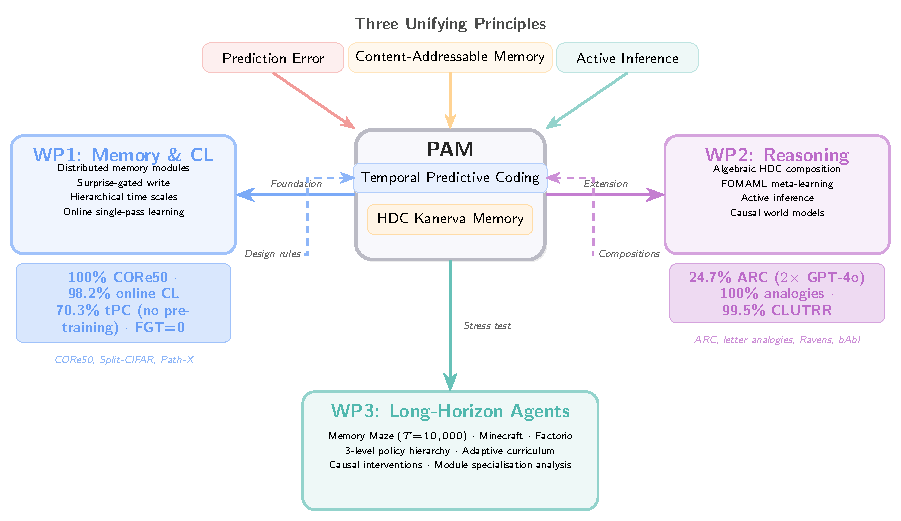
\includegraphics[trim=0mm 0mm 0mm 0mm, clip, width=0.50\textwidth]{figures/overview-find.pdf}
    \caption{\textbf{Conceptual overview of FIND.} PAM (centre) unifies temporal predictive coding, HDC-based content-addressable memory, and active inference under one prediction-error objective. Three work packages build outward: \textbf{WP1} establishes the memory and continual learning foundation; \textbf{WP2} extends with compositional reasoning and causal world models; \textbf{WP3} stress-tests in demanding long-horizon environments. Preliminary results (coloured boxes) validate each WP's core claims.}\label{fig:overview}
    \vspace{-4mm}
\end{wrapfigure}

We live in time. Memory bridges past and present, enabling agents to learn from experience and make informed decisions. Humans develop internal world models for planning and reasoning; replicating this in machines is the next step toward flexible AI~\cite{lecun2022path}.
Current AI struggles to generalise~\cite{razeghi2022impact}, lacking long-term memory~\cite{pasukonis2022evaluating}, causal understanding~\cite{richens2024robust}, and life-long learning without catastrophic forgetting~\cite{wang2024comprehensive}.

Consider an agent managing a Factorio production chain (Figure~\ref{fig:factorio}). It discovers copper wire requires copper plates (step~2,000) and circuits require wire plus iron (step~8,000), then encounters a blueprint requiring 50 circuits at step~15,000. It must recall the dependency chain across $>$10,000 timesteps, reason causally about bottlenecks, and adapt its layout. Current systems cannot do this: transformers trained from experience reach only $\sim$1{,}500-step memory and fail at long-horizon credit assignment~\cite{ni2023longterm}; SSMs compress dependencies into fixed-size state~\cite{gu2021s4}; MANNs lack causal models to identify bottlenecks~\cite{graves2016dnc}. The challenge is to achieve this \textit{learned from raw experience}, without a pretrained model or hand-engineered memory plumbing. \textbf{How can systems intelligently select what to retain, discard, and retrieve to learn across long temporal sequences?}

\begin{figure}[h!]
  \centering
  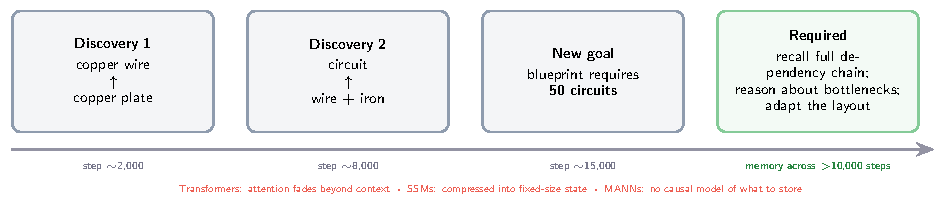
\includegraphics[width=\textwidth]{figures/factorio-storyboard.pdf}
  \caption{\textbf{The capability gap FIND addresses.} An agent discovers dependencies thousands of steps apart and must later recall and compose them under a new goal. This requires selective storage, content-addressable recall, and causal reasoning across $>$10,000 timesteps---beyond current architectures (bottom).}\label{fig:factorio}
\end{figure}

\subsection{Ground-breaking nature and impact}

FIND rests on a single bet: that predictive coding over distributed, content-addressable memory---the brain's mechanism for selective long-horizon recall---is the substrate flexible AI is missing. We develop \textbf{PAM} (\textbf{P}redictive \textbf{A}ctive \textbf{M}emory), a flat modular architecture built on one principle: \textbf{minimising prediction error over a shared memory}. That memory is a content-addressable distributed store~\cite{wu2018kanerva,kanerva2003sparse} whose contents are hyperdimensional vectors~\cite{kanerva2009hyperdimensional}, so recall and symbolic composition (binding, superposition) share one space. Every other mechanism is a way of touching that memory:
\begin{itemize}[noitemsep,topsep=2pt]
  \item \textbf{Encode:} temporal predictive coding denoises each observation into a clean latent before it is stored, so memory holds high-SNR content rather than raw input.
  \item \textbf{Retrieve:} content-addressable read by similarity, with HDC binding making retrieval compositional and symbolic.
  \item \textbf{Act:} active inference selects actions that bring incoming input into line with what memory predicts~\cite{friston2010free,rao2023active}, closing the perception--action loop on the same objective while gathering experience that updates memory.
\end{itemize}
\noindent Learned routing orchestrates which modules read and write when. The name is the thesis: a \textbf{P}redictive, \textbf{A}ctive \textbf{M}emory---predictive coding encodes, active inference acts, and content-addressable read retrieves.

\noindent\textbf{FIND's novelty} is this unification: it sits at the intersection of three established fields in a configuration no prior system has achieved simultaneously:
\begin{itemize}[noitemsep,topsep=2pt]
  \item \textbf{Temporal predictive coding}~\cite{millidge2024temporal} with \textbf{distributed external memory}---not just recurrent state: prior tPC models store context solely in hidden activations; FIND externalises memory into content-addressable HDC slots persistent across thousands of timesteps.
  \item \textbf{Memory-augmented networks}~\cite{graves2016dnc} with \textbf{biologically-grounded iterative inference}---not single-pass read/write: prior MANNs use a single forward pass to address memory; FIND uses iterative predictive-coding inference to resolve ambiguous queries against a content-addressable substrate (94\% exact recall at 32 stored pairs).
  \item \textbf{Hyperdimensional computing}~\cite{kanerva2009hyperdimensional} \textbf{embedded as the storage format of a gradient-trained system}---not as a standalone symbolic method: prior HDC systems operate outside neural training loops, and even NVSA~\cite{hersche2023nvsa}, which couples vector-symbolic reasoning to a trained perception network, is a single-task inference pipeline without persistent temporal memory, continual learning, or action; FIND makes HDC the storage substrate of a continual, temporal system, integrating binding directly into the memory update.
\end{itemize}

\noindent Table~\ref{tab:positioning} situates FIND against the state of the art: no existing system unites these capabilities in one end-to-end trainable architecture.

\begin{table}[h!]
\centering\footnotesize
\caption{\textbf{Positioning of PAM against existing approaches.} Only PAM combines external distributed memory, iterative inference, symbolic binding, and active inference in a single end-to-end trainable architecture.}\label{tab:positioning}
\vspace{2pt}
\begin{tabularx}{\textwidth}{@{}Xcccc@{}}
\toprule
\textbf{System} & \textbf{External Memory} & \textbf{Iterative Inference} & \textbf{Symbolic Binding} & \textbf{Active Inference} \\
\midrule
NTM / DNC~\cite{graves2014ntm,graves2016dnc} & \checkmark & --- & --- & --- \\
Kanerva Machine~\cite{wu2018kanerva} & \checkmark & --- & --- & --- \\
Temporal PC~\cite{millidge2024temporal} & --- & \checkmark & --- & --- \\
HDC systems~\cite{kanerva2009hyperdimensional} & --- & --- & \checkmark & --- \\
S4 / Mamba~\cite{gu2021s4} & --- (compressed state) & --- & --- & --- \\
Titans~\cite{behrouz2025titans} & \checkmark & --- & --- & --- \\
NVSA~\cite{hersche2023nvsa} & --- & --- & \checkmark & --- \\
Active PC~\cite{rao2023active} & --- & \checkmark & --- & \checkmark \\
\textbf{PAM (FIND)} & \textbf{\checkmark} & \textbf{\checkmark} & \textbf{\checkmark} & \textbf{\checkmark} \\
\bottomrule
\end{tabularx}
\end{table}

\subsection{State of the art, knowledge needs, and project objectives}

\subsubsection*{Temporal memory and predictive coding}

A key challenge in AI is creating memory systems comparable to the brain. RAG~\cite{lewis2020retrieval,yuan2024rag} and agentic systems like MemGPT~\cite{packer2024memgpt} manage context through external plumbing, but these sidestep bottom-up lifelong learning and struggle with out-of-distribution scenarios~\cite{razeghi2022impact}.

The core challenge is separating memory storage from computation~\cite{gemici2017generative,gallistel2011memory}. MANNs---NTMs~\cite{graves2014ntm}, DNCs~\cite{graves2016dnc}, Kanerva Machines~\cite{wu2018kanerva}---address this partially. HDC extends sparse distributed memories with symbolic binding~\cite{kanerva2009hyperdimensional,ma2022hyperbox}. Long-context transformers (Infini-Attention~\cite{munkhdalai2024infini}) extend windows but do not solve selective storage. Modern SSMs---Mamba-2~\cite{dao2024mamba2}, xLSTM~\cite{beck2024xlstm}---achieve efficient sequence processing but compress into fixed-size state.

Predictive coding (PC) minimizes prediction errors between expectations and inputs~\cite{millidge2022theoretical,friston2010free}. Extensions to active~\cite{rao2023active} and temporal PC~\cite{millidge2024temporal} enable biologically plausible cognitive maps. Test-time training (TTT)~\cite{sun2024ttt} shares PAM's iterative adaptation principle but modifies the full model rather than memory slots. Titans~\cite{behrouz2025titans} is closest in spirit: it gates test-time writes to a long-term memory by surprise---sharing PAM's write-gating principle---but stores into a monolithic parametric memory without symbolic binding, compositional retrieval, or action selection. \textbf{However, current PC models rely on Markov assumptions, unable to handle long-term credit assignment.}

\subsubsection*{Causal reasoning, world models, and compositional understanding}

A causal world model represents generative mechanisms enabling counterfactual reasoning~\cite{scholkopf2021causal,richens2024robust}. Recent models---JEPA~\cite{drozdov2024jepa}, DINO-WM~\cite{zhou2024dinowm}, GAIA-1~\cite{hu2023gaia1}---show promise, but current benchmarks operate at irrelevant timescales: 2000 steps~\cite{deng2023structured} vs.\ desert ants maintaining memories across 200\,000 steps~\cite{piantadosi2024desert}.

A complementary gap is \textit{compositional reasoning}: factorizing knowledge into reusable subspaces for novel recombinations. The ARC benchmark~\cite{chollet2019arc} exemplifies this---tasks require recognising that transformations \textit{compose} algebraically. FIND addresses this through HDC binding (bind, unbind, superposition) within the same space used for memory.

Cognitive map learning has been pursued in neuroscience~\cite{hafting2005grid} and AI~\cite{whittington2020tolman}, including by our lab~\cite{schoyen2023coherently,pettersen2024elife,pettersen2024nips,schoyen2025plos}, but these lack a unified theory of perception, cognition, and action---the gap FIND addresses.

\subsubsection*{Adaptive learning}

Life-long learning requires managing information without catastrophic forgetting. Current approaches span regularization, replay, and Bayesian methods~\cite{wang2024comprehensive,nguyen2017vcl}; we have explored generative stability~\cite{wasiluk2023genreplay}. FIND addresses this through HDC~\cite{kanerva2009hyperdimensional}: binding memories as compositional vectors enables fast retrieval and symbolic queries without retraining.

\subsection{Research strategy and objectives}

\textbf{Central hypothesis:} Predictive coding over content-addressable distributed memory slots is sufficient for selective long-horizon recall---the ability to store, retrieve, and compose information across thousands of timesteps without catastrophic forgetting---and achieves it where compressed-state methods cannot without unbounded state growth. We decompose this into three testable sub-hypotheses:
\begin{itemize}[noitemsep,topsep=2pt]
  \item \textbf{H1 (WP1):} Non-parametric HDC-structured memory is immune to parameter-overwriting forgetting \textit{by construction}---a guarantee gradient-based methods do not offer---while maintaining competitive accuracy; our CORe50-NI results (92.5\% class-incremental, above a gradient-trained replay head, frozen features) confirm the accuracy side.
  \item \textbf{H2 (WP2):} Compositional binding in HDC space enables zero-shot generalisation to novel transformation compositions, with distributed memory as a load-bearing component of test-time program synthesis---PAMNCA ablations attribute 30--43\% of performance to memory, growing with compute budget.
  \item \textbf{H3 (WP3):} Memory-augmented agents outperform compressed-state agents (SSMs, Transformers) specifically on tasks requiring recall across $>$5,000 timesteps.
\end{itemize}

\noindent H1--H3 concern the memory itself (encode, retrieve); the third operation, \textit{act} (active inference), extends the same objective to action and is a design principle developed in WP2--3, not a Part~I claim. We address these through three objectives and corresponding work packages:

\begin{itemize}[noitemsep,topsep=2pt]
  \item \textbf{Objective 1 / WP1: Temporal Predictive Coding with Distributed Memory.} Develop the foundational PAM architecture that processes information over different time scales through temporal predictive coding with distributed memory modules.
  \item \textbf{Objective 2 / WP2: Causal Reasoning and Compositional Understanding.} Extend PAM with active inference, neurosymbolic integration, and subspace-based compositional reasoning for causal world model learning.
  \item \textbf{Objective 3 / WP3: Long-Horizon Adaptation in Open-Ended Environments.} Stress-test the complete PAM system across a graduated suite of environments---Memory Maze, then Minecraft, with Factorio as the aspirational capstone---that require sophisticated planning, resource management, and long-horizon adaptation.
\end{itemize}

\noindent\textbf{Theoretical approach.} A shared content-addressable memory (Kanerva store~\cite{wu2018kanerva}, HDC format) sits at PAM's centre; three processes read and write it under one prediction-error objective:
\begin{enumerate}[noitemsep,topsep=2pt]
  \item \textit{Encode:} temporal predictive coding iteratively refines each latent, so the denoised estimate---not the raw input---is what is written.
  \item \textit{Retrieve \& compose:} modules read by content similarity, with HDC binding making retrieval compositional; module specialization is set by Gumbel-softmax routing applied iteratively over $n$ stages.
  \item \textit{Act:} active inference selects actions that drive inputs toward memory-derived predictions---reducing uncertainty (exploration) and storing causally relevant experience.
\end{enumerate}

\noindent Retrieval uses similarity between $z^m_t$ and stored basis vectors $h^m_i$, with exponential maps~\cite{pettersen2025exponential} giving closed-form Riemannian updates on the memory manifold (Figure~\ref{fig:arch}).

\begin{figure}[ht]
  \centering
  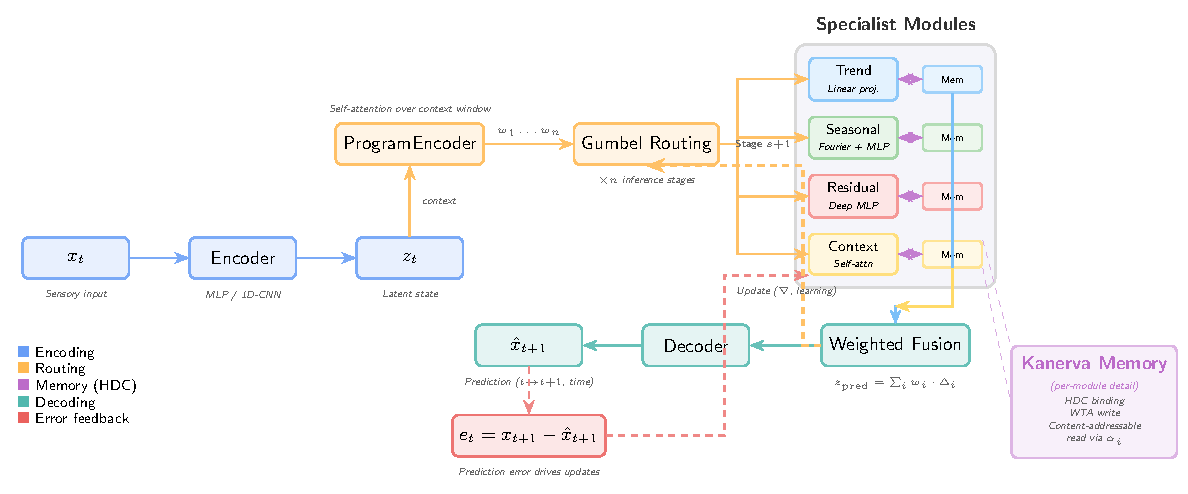
\includegraphics[width=\textwidth, clip]{figures/pam-architecture.pdf}
  \caption{\textbf{PAM architecture.} Sensory input $x_t$ is encoded into latent state $z_t$. A ProgramEncoder infers routing weights via self-attention over the context window. Gumbel-softmax routing selects among four specialist modules (Trend, Seasonal, Residual, Context), each with dedicated Kanerva memory using HDC binding for content-addressable read/write. The routing is applied iteratively over $n$ stages. Module outputs are fused into a prediction $\hat{x}_{t+1}$; prediction errors drive parameter updates. The module inventory is task-dependent (shown here for temporal forecasting).}\label{fig:arch}
\end{figure}

\noindent\textit{Preliminary results.}
The BioAI group has developed FIND's foundations through neurocomputational memory research: grid/place/border cells emerge spontaneously in AI agents~\cite{schoyen2023coherently}, orthogonal remapping encodes context~\cite{pettersen2024nips,schoyen2025plos,pettersen2024elife}, NCA enables self-organizing module communication~\cite{kvalsund2026sensor}, one-shot memory transfer~\cite{guichard2025engramnca}, and abstract reasoning~\cite{guichard2025arc}. On the memory substrate itself, a Kanerva/HDC store gives \textbf{94--95\% exact associative recall} at 32 stored pairs ($D{=}512$), with interference following the vector-symbolic capacity law ($0.94/0.59/0.39$ at $K{=}32/64/96$; Figure~\ref{fig:prelim})---a mechanism verification that grounds, but does not yet substitute for, task-level recall.

\textbf{WP1: Memory and continual learning.} On the official CORe50-NI online continual-learning protocol (single pass, no gradient updates on the stream, no task boundaries), PAM's unified gradient-free memory---surprise-gated exemplars, prototypes, and streaming class statistics in one architecture---reaches \textbf{92.5\% class-incremental accuracy} over frozen self-supervised (DINOv2) features with \textbf{$\approx$0 forgetting by construction}, above a gradient-trained replay head (87.7\%); accuracy scales cleanly with memory budget ($65.2{\to}74.7{\to}83.3\%$ at $16{\to}64{\to}256$ exemplars/class) and reaches \textbf{92.8\% on CLEAR-10} and \textbf{78.4\% on Split-CIFAR-100} (3 seeds; deterministic readouts reproduce to four decimals). These use a \textit{frozen} backbone. Learning the representation \textit{from raw experience}---FIND's ambition---does not yet work: an online tPC encoder collapses to chance, a failure mode we have diagnosed to detached-target amortized objectives (linear probe $0.02$ vs $0.29$ for a random encoder). We therefore make zero-pretraining online representation learning an explicit \textbf{WP1 objective} (reconstruction/contrastive anchoring + a streaming readout) rather than a solved capability, and report only frozen-backbone numbers as demonstrated.

\begin{wrapfigure}{l}{0.6\textwidth}
  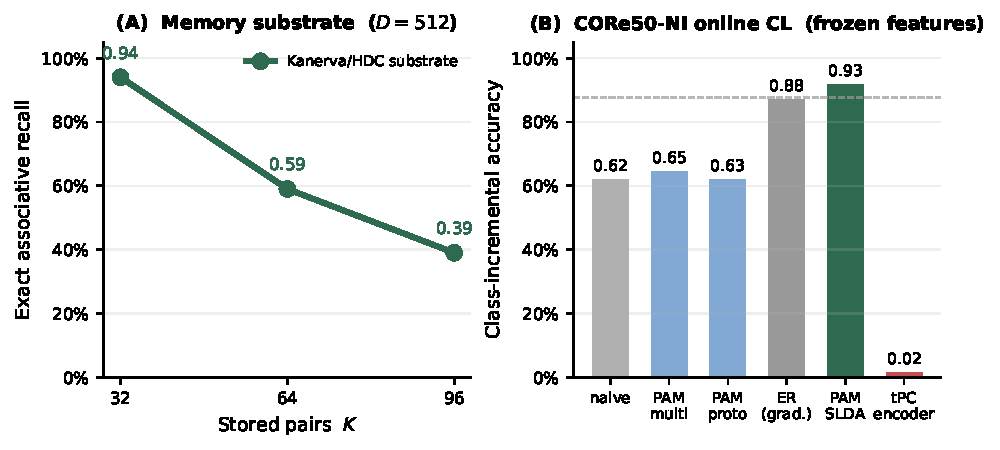
\includegraphics[width=0.99\linewidth,keepaspectratio=true]{figures/prelim_results.pdf}
  \caption{\textbf{Preliminary PAM results (WP1 foundation).}
    (A)~Exact associative recall of the Kanerva/HDC substrate vs.\ number of stored pairs $K$: $0.94/0.59/0.39$ at $K{=}32/64/96$ ($D{=}512$), matching vector-symbolic capacity theory---a mechanism check, not yet a task-level result.
    (B)~Online class-incremental accuracy on CORe50-NI (single pass, frozen DINOv2 features): the unified gradient-free memory reaches $92.5\%$ with $\approx$0 forgetting, above a gradient-trained replay head, and scales with memory budget. From-scratch (tPC-encoder) representation learning collapses to chance---a WP1 objective, not a result.}\label{fig:prelim}
  \vspace{-3mm}
\end{wrapfigure}

\textbf{WP2: Compositional reasoning.} On the Abstraction and Reasoning Corpus (ARC)~\cite{chollet2019arc}, our PAMNCA system---a neural cellular automaton with distributed PAM memory (1.47M parameters), no pretrained backbone---reaches \textbf{40\% exact match} (leave-one-out over the 400 training tasks; $510$--$530/1302$ episodes across seeds) via meta-learned initialisation and batched test-time training, up from 24.7\% in an earlier configuration, and \textbf{26.4\% on the fully held-out evaluation split} (in progress)---evidence that the mechanism is task-general adaptation, not memorisation. The significance is the efficiency frontier: large program-synthesis ensembles exceed this only with $10^5$--$10^6\times$ more compute, whereas PAMNCA reaches it at $>$1000$\times$ fewer parameters, learning each task from its support examples alone. Memory ablations attribute \textbf{30--43\%} of performance to the distributed memory, growing with compute budget. A two-sided negative sharpens the plan: low-rank (LoRA) program composition fails, and a one-shot HDC program encoder generalises to only 29\% on held-out 2-step compositions---compositional \textit{representation} does not buy compositional \textit{inference}, motivating the iterative/resonator encoding of T2.2.

\begin{figure}[h!]
  \centering
  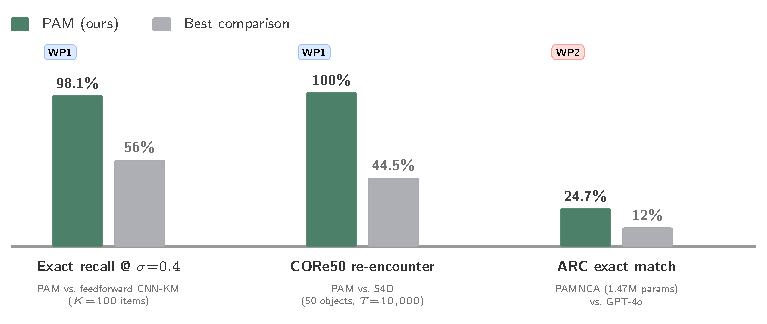
\includegraphics[width=.9\textwidth]{figures/headline-results.pdf}
  \caption{\textbf{Headline preliminary results.} PAM on each benchmark: exact associative recall of the memory substrate (94\% @32 pairs, WP1 foundation), online class-incremental accuracy on CORe50-NI (92.5\%, frozen features, above a gradient-trained replay head, WP1), and ARC program synthesis via test-time training (40\% leave-one-out, 26\% held-out, WP2).}\label{fig:headline}
\end{figure}

Two sub-hypotheses already have preliminary support: (1)~non-parametric memory yields $\approx$0 \textit{additional} forgetting by construction while remaining competitive---92.5\% class-incremental on CORe50-NI, above a gradient-trained replay head; (2)~distributed memory is load-bearing for test-time program synthesis---PAMNCA ablations attribute 30--43\% of ARC performance to memory. The third capability, zero-pretraining online representation learning, is falsified in its naive form (tPC collapse) and becomes a concrete WP1 objective---a design target, not a claim.

\subsection{Major expected outcomes}

\noindent\textbf{Science:} A theoretical framework in which perception, memory, and action reduce to one prediction-error objective, extending predictive coding beyond its Markovian limits. Understanding of how modular specialization emerges from predictive principles.

\noindent\textbf{Technology:} PAM as open-source framework with benchmarks spanning forecasting (ETT, Weather), long-range memory (Path-X, Memory Maze), and continual learning. Orchestration algorithms with reproducible evaluation suites.

\noindent\textbf{Society:} Foundations for AI with principled memory applicable to healthcare (patient timelines), industrial automation (Factorio-style planning), and environmental monitoring.

\noindent\textbf{Success criteria:} (i)~class-incremental accuracy matching a gradient-trained replay baseline on CORe50-NI/CLEAR-10 at $<$10\% of its compute, plus a working \textit{zero-pretraining} online readout ($>$70\% on CORe50-NI) (WP1); (ii)~competitive exact-match on \textbf{ARC-AGI-2} at $<$10M parameters with no pretrained backbone---baseline 40\% (ARC-AGI-1 leave-one-out) / 26\% held-out---with interactive \textbf{ARC-AGI-3} as a stretch target (WP2); (iii)~$>$10\,pp over a parameter-matched LSTM on the Memory-Maze diagnostic, then exploration/transfer above an LSTM agent on ARC-AGI-3 (WP3). Team: PI (50\%), one postdoc (ML systems), two PhDs; 4-tier benchmark hierarchy (Part~II).

\printbibliography[title={References}]

}

{\setstretch{1.0}
% ============================================================
% CURRICULUM VITAE AND TRACK RECORD (max. 4 pages)
% ============================================================
% Header: Lepperød — FIND — Part B1

\newpage
\section{Curriculum Vitae and Track Record}

\subsection*{Personal details}

\begin{tabular}{ll}
\textbf{Name:} & Dr.\ Mikkel Elle Lepperød \\
\textbf{Date of birth:} & 14 September 1985 \\
\textbf{Nationality:} & Norwegian \\
\textbf{ORCID:} & 0000-0002-4262-5549 \\
\textbf{URL:} & \url{https://www.simula.no/people/mikkel} \\
\end{tabular}

\subsection*{Education and key qualifications}

\begin{tabular}{lp{12cm}}
2020 & \textbf{Ph.D.}\ Neuroscience, Faculty of Medicine, University of Oslo, Norway \\
2014 & \textbf{M.Sc.}\ Applied Mathematics, Norwegian University of Life Sciences, Norway \\
\end{tabular}

\subsection*{Current and relevant previous positions}

\begin{tabular}{lp{12cm}}
2026-- & \textbf{Senior Research Scientist} (equiv.\ associate professor), Simula Research Laboratory \\
2023-- & \textbf{Adjunct Associate Professor} (20\%), Dept.\ of Physics, University of Oslo \\
2022--2026 & \textbf{Research Scientist} (equiv.\ assistant professor), Simula Research Laboratory \\
2020--2022 & \textbf{Postdoctoral Fellow}, Dept.\ of Biosciences, University of Oslo \\
\end{tabular}

\noindent\textbf{PhD supervisor:} Prof.\ Torkel Hafting and Prof.\ Marianne Fyhn (University of Oslo). \\
\textbf{Postdoctoral mentor:} Self-directed (group leader from 2020).

\noindent\textbf{Career breaks:} Parental leave (5 months in 2017, 5 months in 2020).

\subsection*{Research outputs}

The following ten outputs demonstrate my trajectory from experimental neuroscience to neuro-inspired AI, establishing the foundations for FIND:

\begin{enumerate}[noitemsep,topsep=2pt]
  \item \textbf{Lepperød ME}, Christensen AC, Lensjø KK, Buccino AP, Yu J, Fyhn M, Hafting T. \textit{Optogenetic pacing of medial septum parvalbumin-positive cells disrupts temporal but not spatial firing in grid cells}. Science Advances, 2021.
  \textit{Role: First author, conceived and led the study. Significance: Established causal evidence for temporal coding in the entorhinal cortex, directly motivating the temporal predictive coding component of PAM.}

  \item \textbf{Lepperød ME}, Stöber T, Hafting T, Fyhn M, Kording KP. \textit{Inferring causal connectivity from pairwise recordings and optogenetics}. PLoS Computational Biology, 2023.
  \textit{Role: First author. Significance: Developed quasi-experimental methods for causal inference in neural circuits, grounding FIND's causal reasoning objectives.}

  \item Schøyen VS$^*$, Pettersen MB$^*$, Holzhausen K, Fyhn M, Malthe-Sørenssen A, \textbf{Lepperød ME}. \textit{Coherently remapping toroidal cells but not grid cells are responsible for path integration in virtual agents}. iScience, 2023.
  \textit{Role: Senior/corresponding author, supervised the project. Significance: Showed that AI agents spontaneously develop biologically consistent spatial cells, establishing our lab's cognitive map expertise.}

  \item Pettersen MB, Schøyen VS, Malthe-Sørenssen A, \textbf{Lepperød ME}. \textit{Learning place cells and remapping by decoding the cognitive map}. eLife, 2025.
  \textit{Role: Senior/corresponding author. Significance: Demonstrated context-dependent memory through orthogonal remapping, key to FIND's modular memory design.}

  \item Pettersen MB, Rogge F, \textbf{Lepperød ME}. \textit{Learning place cell representations and context-dependent remapping}. NeurIPS, 2024.
  \textit{Role: Senior author. Significance: Extended cognitive map learning to context-switching, directly informing WP2's compositional reasoning.}

  \item Kvalsund MK, Ellefsen KO, Glette K, Pontes-Filho S, \textbf{Lepperød ME}. \textit{Sensor movement drives emergent attention and scalability in active neural cellular automata}. Neural Networks, 2026.
  \textit{Role: Senior/corresponding author. Significance: Demonstrated NCA-based inter-module communication with active vision---the primary orchestration mechanism for PAM.}

  \item Guichard E, Reimers F, Kvalsund MK, \textbf{Lepperød M}, Nichele S. \textit{EngramNCA: A neural cellular automaton model of memory transfer}. ALife, 2025.
  \textit{Role: Co-supervisor. Significance: Showed NCA-based one-shot memory transfer between modules, directly enabling PAM's distributed memory architecture.}

  \item Guichard E, Reimers F, Kvalsund MK, \textbf{Lepperød M}, Nichele S. \textit{ARC-NCA: Towards developmental solutions to the Abstraction and Reasoning Corpus}. ALife, 2025. Featured on Machine Learning Street Talk podcast.
  \textit{Role: Co-supervisor. Significance: Demonstrated abstract reasoning through developmental self-organization, informing WP2's compositional reasoning.}

  \item Schøyen VS, Beshkov K, Pettersen MB, Hermansen E, Holzhausen K, Malthe-Sørenssen A, Fyhn M, \textbf{Lepperød ME}. \textit{Hexagons all the way down: Grid cells as a conformal isometric map of space}. PLOS Computational Biology, 2025.
  \textit{Role: Senior/corresponding author. Significance: Provided geometric theory of neural representations, informing HDC integration in PAM.}

  \item Danielli K, \textbf{Lepperød ME}. \textit{A bio-inspired minimal model for non-stationary K-armed bandits}. Biological Cybernetics, 2026.
  \textit{Role: Senior/corresponding author. Significance: Demonstrated bio-inspired adaptive learning under non-stationarity, directly relevant to WP3's open-ended adaptation.}
\end{enumerate}

\subsection*{Significant peer recognition}

\begin{itemize}[noitemsep,topsep=2pt]
  \item \textbf{NORA Award for Early Career Investigator} (2025)---National recognition for contributions to NeuroAI
  \item \textbf{Simula ERC Incubator} (2022)---Selected for institutional support program for ERC candidates
  \item \textbf{Wharton Executive Education} (2022)---``High-Potential Leaders: Accelerating Your Impact''
  \item \textbf{Invited speaker}: University of California San Diego (2022), AI Week Oslo Met (2023), Keynote at Young Researchers in NeuroAI (2023), Simula Bio-inspired Computing Seminar (2024)
  \item \textbf{Workshop organizer}: 4-day NeuroAI workshop on Hurtigruten with 20 international speakers (2024); co-organizer of 3+ NeuroAI workshops connecting national and international labs (2023--2024)
  \item \textbf{Reviewer}: Nature Machine Intelligence, PLoS Computational Biology, eNeuro
  \item \textbf{Board member}: NORA Special Interest Group for NeuroAI Norway
  \item \textbf{Public outreach}: Brain Inspired podcast (2024), Machine Learning Street Talk podcast (2025), NRK interview (2021), opinion pieces in digi.no and forskning.no
\end{itemize}

\subsection*{Project leadership and supervision}

\noindent\textbf{Group leader, BioAI group at Simula} (2020--present): 4.5 MNOK/year, managing 3 PhD students, 1 postdoc. Built the group from inception to a productive research unit with publications at NeurIPS, eLife, Science Advances, and Nature Communications.

\noindent\textbf{Acting co-PI, Bio-inspired neural networks for AI application} (2020--2026): 16 MNOK RCN-funded project, University of Oslo. Co-supervised 3 PhDs.

\noindent\textbf{Supervised to completion}: 2 PhD students (V.\ Schøyen, K.\ Holzhausen), 8+ MSc students (including graduates now at Stanford PhD program and UiO PhD program).

\subsection*{Research software and ML systems engineering}

\noindent\textbf{PAM / PAMNCA codebases:} Large-scale ML engineering behind the preliminary results in this proposal: systematic GPU-cluster experimentation ($\sim$15K GPU-hours on A40s), automated result parsing from 150+ log files, reproducible evaluation pipelines, and continual-learning benchmarking on CORe50 using the official online (NI) protocol.

\noindent\textbf{Community research infrastructure:} Co-developed NEST simulator modules within the Human Brain Project; co-developed the Exdir hierarchical data format and the Expipe experiment-management platform for reproducible neuroscience pipelines.

\noindent\textbf{Benchmark contributions:} Evaluation on official public protocols (CORe50-NI, ARC).

\noindent\textbf{Team profile to complement the PI:} The FIND postdoc will be recruited from the ML systems community (target profile: PhD from an ICLR/ICML-publishing lab with large-scale training experience) to complement the PI's neuroscience background and own the WP2--3 scaling infrastructure.

\subsection*{Additional information}

\noindent\textbf{Community leadership}: Lead role establishing NeuroAI as focus field in the Norway--US Ministry of Education collaboration (2022). Developed and taught the NeuroAI course at University of Oslo (2023).

}

\end{refsection}

% ============================================================
% PART B2: Part II of the Scientific Proposal
% ============================================================
\newpage
\switchtobtwo
% Part II is submitted as a separate PDF (B2); restart figure/table numbering
% so the split B2 is self-contained. Cross-refs to Part I resolve via \ref
% (label numbers are captured at figure creation, before this reset).
\setcounter{figure}{0}
\setcounter{table}{0}
\begin{refsection}

{\setstretch{1.0}
% ============================================================
% PART II OF THE SCIENTIFIC PROPOSAL (max. 7 pages)
% References do not count towards the page limit.
% ============================================================
% Header: Lepperød — FIND — Part B2

\section{Part II of the Scientific Proposal}

This section details the research methodology, work plan, and risk assessment for FIND. Part II complements Part I by providing the implementation specifics; it should not be read as a repetition of Part I but as a detailed elaboration of how the objectives will be achieved.

\textbf{Research questions:}
\begin{itemize}[noitemsep,topsep=2pt]
  \item Q1: How can memory-augmented modules distribute and combine long-term temporal information?
  \item Q2: How can such modules support active inference and causal reasoning?
  \item Q3: How can neurosymbolic components be integrated into distributed memory architectures without sacrificing gradient-based learning?
  \item Q4: Does this integration measurably enhance compositional reasoning in complex environments?
  \item Q5: Can such networks learn adaptively and reason about causal relations over long time horizons?
\end{itemize}

\subsection{Research methodology}

The core update equations underpin PAM's mechanisms. Each module $m$ has latent state $z^m_t \in \mathbb{R}^{d_z}$ and sensory input $x^m_t \in \mathbb{R}^{d_x}$ at time $t$. The prediction error $e_t = x^m_t - \hat{x}^m_t$ drives module state updates: $z^m_{t+1} = f_m(z^m_t, c^m_t, r^m_t, a_t)$, where $f_m$ is a learnable function, $a_t$ is the action, $r^m_c = \sum_i \alpha^m_c[i]h^m_i$ is context-dependent memory retrieval, and $c^m_t$ is contextual input from inter-module communication. Two primary orchestration mechanisms will be explored:
\begin{enumerate}[noitemsep,topsep=2pt]
  \item \textbf{\textit{Message passing:}} attention and convolution combined with aggregation---demonstrated in active vision~\cite{kvalsund2026sensor}
  \item \textbf{\textit{Neural cellular automata (NCA):}} self-organizing principles for module communication---demonstrated in one-shot memory transfer~\cite{guichard2025engramnca} and abstract reasoning~\cite{guichard2025arc}
\end{enumerate}
\noindent We commit to \textbf{NCA + message passing} as the primary orchestration mechanisms, supported by our PAMNCA results where NCA + distributed memory outperforms no-memory variants by 30--43\%. Four further mechanisms form a structured ablation ladder in WP2: \textit{Hypernetwork}, \textit{Predictive routing}, \textit{Competitive collaboration}, and \textit{Energy-based orchestration}---ordered by increasing biological plausibility and implementation complexity.

\subsubsection*{WP1: Temporal Predictive Coding with Distributed Memory \textnormal{(Lepperød, PhD1; Q1; Years 1--3)}}

WP1 establishes the core PAM architecture for temporal prediction and memory. Building on our preliminary results ($98.1\%$ exact recall at $\sigma{=}0.4$, $3.75{\times}$ less forgetting than tPC-alone), WP1 extends the architecture to challenging temporal benchmarks and characterizes its operational regime.

\noindent\textbf{Benchmark strategy.} We adopt a four-tier evaluation hierarchy designed to systematically validate PAM's capabilities and position it against the state of the art:
\begin{itemize}[noitemsep,topsep=2pt]
\item \textbf{Tier~1 --- Validation:} Synthetic tasks (Copy Task $T{=}100$--$5{,}000$; Adding Problem) and our existing MNIST/Omniglot benchmarks. These confirm core memory mechanisms work before scaling.
\item \textbf{Tier~2 --- Field positioning:} Standard time series forecasting benchmarks (ETT, Weather, ECL, Traffic) at horizons $\{96, 192, 336, 720\}$. Compared against DLinear, PatchTST~\cite{nie2023patchtst}, iTransformer~\cite{liu2024itransformer}, and Mamba using MSE/MAE metrics. These establish PAM's competitiveness with purpose-built forecasting models.
\item \textbf{Tier~3 --- Core thesis:} Long-range benchmarks that test PAM's distinctive claims. Sequential MNIST ($T{=}784$), Long Range Arena~\cite{tay2021lra} including Path-X ($T{=}16{,}384$), Memory Maze~\cite{pasukonis2022evaluating} ($T{=}2{,}000$--$10{,}000$), and infinite dSprites~\cite{dziadzio2023infinite} ($T{=}2{,}000$--$50{,}000$). If PAM achieves above-chance on Path-X, it demonstrates that HDC memory can compete with SSMs on ultra-long-range tasks.
\item \textbf{Tier~4 --- Continual learning:} Split MNIST/CIFAR (5 sequential tasks), concept drift benchmarks, and TSCIL~\cite{tscil2023} for time series class-incremental learning. These test whether PAM's memory consolidation prevents catastrophic forgetting.
\end{itemize}

\begin{figure}[ht]
  \centering
  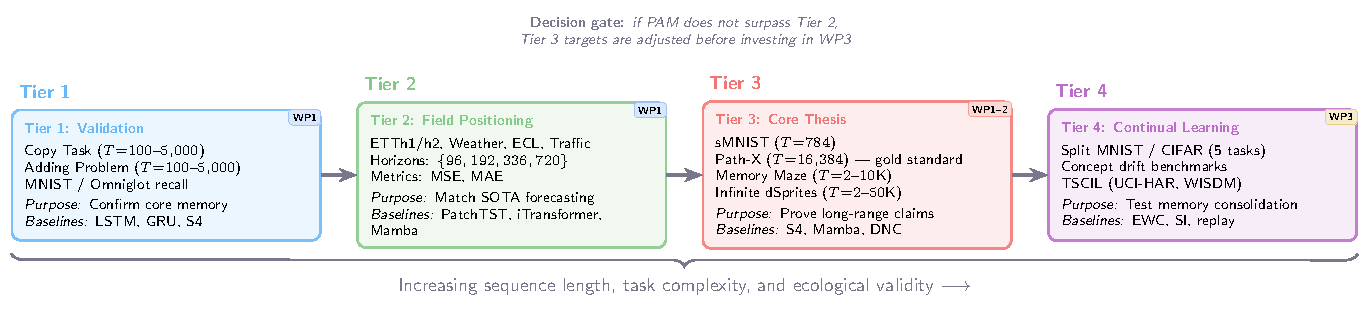
\includegraphics[width=\textwidth, clip]{figures/benchmark-tiers.pdf}
  \caption{\textbf{Four-tier benchmark hierarchy for PAM evaluation.} Increasing sequence length, task complexity, and ecological validity from left to right. WP badges indicate which work package addresses each tier. A decision gate between Tiers~2 and 3 ensures incremental validation before committing to the most ambitious benchmarks.}\label{fig:tiers}
\end{figure}

\paragraph{T1.1: Temporal Benchmarks and Architecture Scaling}
\textbf{Completed:} MNIST digit recall benchmark~\cite{gemici2017generative} (see Part I, Fig.~3).
\textbf{Planned:} Validate on Tier~1 (Copy Task, Adding Problem) and Tier~2 (ETT, Weather, ECL) benchmarks. Visual encoding via ResNet~\cite{he2016resnet}. Compare against GTMs~\cite{gemici2017generative}, VRNNs~\cite{chung2015vrnn}, LSTMs~\cite{hochreiter1997lstm}, S4~\cite{gu2021s4}, NTMs~\cite{graves2014ntm}, and DNCs~\cite{graves2016dnc}. Offline probing~\cite{park2023probing} will analyze learned representations.
\textit{Success criterion:} PAM must achieve ${\ge}90\%$ exact recall at $\sigma{=}0.3$ on Tier~1 tasks and MSE within 10\% of PatchTST on Tier~2.

\paragraph{T1.2: Inference Depth, Noise Robustness, and Capacity}
Systematically characterise the recall--noise--capacity landscape across $\sigma \in [0.0, 0.8]$ and $K \in [10, 500]$. Implement adaptive inference depth via prediction-error thresholding: at each iteration, compare the current prediction error against a learned threshold; terminate early when the error is below threshold, saving computation. Characterise interactions between slot count, HDC dimension, and forgetting rate under varying concept-drift speeds, providing design guidelines for WP2--3.
\textit{Success criterion:} Adaptive inference must achieve ${\geq}95\%$ of full-iteration accuracy at ${\leq}60\%$ of compute on the MNIST benchmark.

\paragraph{T1.3: Hierarchical Temporal Compression for Long-Horizon Memory}
Extend PAM with hierarchical time-scale factorisation: fast modules ($\Delta t{=}1$) process step-level inputs while slow modules compress episodes into semantic summaries via learned gating inspired by complementary learning systems~\cite{ramapuram2021kanerva}. The gating criterion---whether and when prediction error triggers consolidation from episodic to semantic memory---will be resolved experimentally using prediction-error statistics from T1.2. Evaluate on Tier~3 benchmarks: ``infinite dSprites'' ($T{=}2{,}000$--$50{,}000$) and Memory Maze ($T{=}2{,}000$--$10{,}000$)~\cite{pasukonis2022evaluating}. The key test is \textbf{Path-X} ($T{=}16{,}384$): only S4, Mamba, and a few others solve this benchmark; success here would demonstrate that HDC memory with iterative inference can match purpose-engineered SSMs on ultra-long-range tasks.

\subsubsection*{WP2: Causal Reasoning and Compositional Understanding \textnormal{(Lepperød, PD; Q2--Q4; Years 2--4)}}

WP2 extends PAM with active inference, causal world model learning, and subspace-based compositional reasoning. This WP integrates neurosymbolic components for explicit reasoning alongside statistical learning, while enabling the system to discover causal structure through interventions.

\paragraph{T2.1: Action-Augmented Temporal Predictive Coding}
Extend PAM to incorporate action nodes that modulate state transitions. Develop action-dependent prediction error computation across multiple timescales, including action-conditioned memory addressing, action-dependent update rules, and methods for maintaining temporal consistency. Design joint optimization of state predictions and action selections.
\textit{Success criterion:} Action-conditioned prediction error must correlate $r{>}0.7$ with observed state transitions in a controlled navigation task.

\paragraph{T2.2: Subspace Reasoning and Compositional Understanding}
Develop mechanisms for compositional, subspace-based reasoning within the PAM architecture. The core idea is to factorize latent spaces into semantically meaningful subspaces that can be \textit{composed algebraically} through HDC binding operations. Concretely, this means representing transformations as operations that compose exactly: a rotation followed by a colour change should produce the same result whether applied individually or as a single bound operation. Our preliminary PAMNCA results (24.7\% exact match on ARC with 1.47M parameters) validate this approach, and memory ablations show that distributed memory contributes 30--43\% of performance. Importantly, LoRA program decomposition experiments demonstrate that ARC programs are \textit{not} low-rank composable, motivating the shift to HDC algebraic composition which operates in $d{=}1000{+}$ dimensional space with guaranteed compositionality. We will implement: (i)~a lossless per-cell circular embedding for spatial structures; (ii)~algebraically exact primitives (rotation, reflection, translation, colour transformations) that compose via HDC binding; (iii)~a meta-learning pipeline (FOMAML~\cite{finn2017maml}) for few-shot program inference from support examples; and (iv)~HDC program storage enabling compositional search over the space of transformations. We evaluate compositional reasoning on abstract visual reasoning benchmarks including ARC~\cite{chollet2019arc}, letter-string analogies~\cite{mitchell1993analogy}, and bAbI multi-hop QA~\cite{weston2015babi}.
\textit{Success criterion:} Extend PAMNCA from 24.7\% to $>$40\% exact match on ARC through HDC algebraic composition. Compositional retrieval must generalise to out-of-distribution rules (e.g., novel rotation--colour combinations). Our preliminary miniARC search achieves 100\% OOD exact match on 4 novel rules. Figure~\ref{fig:comp} illustrates the approach.

\begin{figure}[ht]
  \centering
  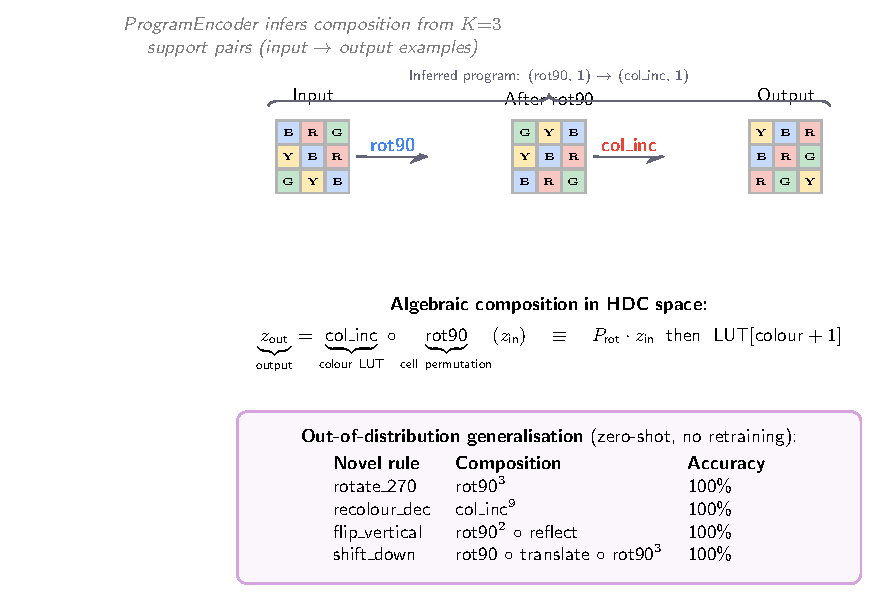
\includegraphics[width=0.85\textwidth, clip]{figures/compositional-reasoning.pdf}
  \caption{\textbf{Compositional reasoning through algebraic operations in HDC space.} A visual transformation (rotation + colour increment) is decomposed into composable primitives. The ProgramEncoder infers the composition from support examples. Algebraic composition guarantees out-of-distribution generalisation to novel rules without retraining (bottom table).}\label{fig:comp}
\end{figure}

\paragraph{T2.3: Causal World Model Learning through Active Inference}
Implement active inference for action selection balancing information gain and goal-oriented reward~\cite{friston2010free,rao2023active}. Develop causal discovery mechanisms through interventionist exploration: the agent executes targeted interventions (changing one variable while holding others fixed), observes the downstream effects, and updates its world model to encode directional causal relationships rather than mere correlations. This follows the ``interventionist'' approach to causal learning~\cite{scholkopf2021causal}: modules learn not just that ``opening a chest produces items'' but that ``the chest \textit{caused} items to appear,'' enabling counterfactual reasoning (``what if I hadn't opened the chest?''). Build on our work with NCA~\cite{kvalsund2024nca,kvalsund2026sensor} and proximal policy optimization~\cite{schulman2017ppo} for credit assignment.
\textit{Success criterion:} PAM with active-inference exploration must reach task completion $2{\times}$ faster than standard PPO on at least two benchmark environments.

\paragraph{T2.4: Orchestration Ablation and Evaluation}
Execute comprehensive ablation studies to quantify the contribution of each orchestration mechanism, distributed memory, and neurosymbolic component. Evaluate PAM on few-shot continuous control~\cite{mete2024few,yu2019meta} and long-horizon planning~\cite{pasukonis2022evaluating}. Investigate how PAM's computations map onto neural circuits by extending our established RNN framework~\cite{schoyen2023coherently,pettersen2024elife,pettersen2024nips} that demonstrates spontaneous development of grid, place, and border cells.
\textit{Success criterion:} PAM must achieve ${>}10$ percentage point improvement over LSTM baseline on Memory Maze ($T{>}500$ steps)---a deliberately intermediate gate; WP3 raises the bar to $T{=}10{,}000$ against stronger baselines (DQN, Dreamer). Orchestration ablations must show primary NCA/message-passing design outperforms at least two alternatives.

\subsubsection*{WP3: Long-Horizon Adaptation in Open-Ended Environments \textnormal{(Lepperød, PhD2; Q4--Q5; Years 3--5)}}

WP3 stress-tests PAM in environments demanding sophisticated planning, resource management, and adaptation to ever-changing dynamics. We adopt a tiered ambition structure:
\begin{itemize}[noitemsep,topsep=2pt]
  \item \textbf{Must achieve:} Memory Maze at $T{=}10{,}000$ with clear improvement ($>$10\,pp) over LSTM/DQN baselines.
  \item \textbf{Should achieve:} Simplified Minecraft tasks (navigation, basic crafting) via Python Malmo API~\cite{johnson2016malmo}.
  \item \textbf{Stretch goal:} Factorio production chains~\cite{kant2025factorio} requiring multi-step resource management across $T{>}10{,}000$ steps.
\end{itemize}

\paragraph{T3.1: Environment Development and Curriculum Design}
Design complex scenarios with varied challenges: resource management, crafting, building, combat, and exploration. Specific task designs include: (i)~Memory Maze~\cite{pasukonis2022evaluating} at increasing horizons ($T{=}2{,}000$--$10{,}000$); (ii)~multi-step crafting chains in Factorio where intermediate products must be stored and recalled across $T{>}10{,}000$ steps; (iii)~spatial exploration in Minecraft where the agent must build a mental map of a procedurally generated environment. Create a procedural generation pipeline varying task complexity, resource constraints, and causal dependencies. Implement adaptive curriculum using automatic curriculum learning~\cite{portelas2020acl} and intrinsic motivation~\cite{aubret2023intrinsic}: task difficulty increases only when the agent's competence (measured via prediction accuracy) exceeds a threshold. Observations via frozen ResNet~\cite{he2016resnet} encoder and game-state variables.

\paragraph{T3.2: Long-Horizon Active Inference Agent}
Integrate PAM into an interactive agent with a three-level policy hierarchy: (L1)~step-level motor primitives via PPO~\cite{schulman2017ppo}---low-level actions like movement, item use, crafting; (L2)~sub-goal selection via hindsight experience replay~\cite{andrychowicz2017her}---mid-level objectives like ``go to location X,'' ``collect item Y''; (L3)~strategic planning as symbolic goal vectors in HDC space~\cite{kanerva2009hyperdimensional,rajendran2024causal}---high-level plans like ``build a shelter before nightfall'' composed from bound sub-goal vectors. Each level maps to PAM modules operating at different temporal scales: L1 uses fast modules ($\Delta t{=}1$), L2 uses medium modules ($\Delta t{=}10$--$100$), and L3 uses slow modules ($\Delta t{=}100$--$1{,}000$) with persistent memory. Co-train through RL and self-supervised prediction objectives.

\paragraph{T3.3: Causal and Adaptive Learning Analysis}
Assess causal learning through interventions (changing game rules, introducing disturbances), counterfactual reasoning (simulating alternative scenarios), and analyzing the agent's ability to predict effects of its actions. Measure module specialization by analyzing activity patterns, stored information types, and task-specific contributions. Compare against DQN~\cite{mnih2015dqn}, PPO, RND~\cite{burda2018rnd}, Dreamer~\cite{hafner2018dreamer}, DINO-WM~\cite{zhou2024dinowm}, and MuZero~\cite{schrittwieser2019muzero}.
\textit{Success criteria:} (i)~PAM achieves $>$10\,pp improvement over DQN on Memory Maze at $T{>}5{,}000$ steps. (ii)~On Minecraft sub-tasks, PAM reaches task completion at least $1.5{\times}$ faster than PPO baseline. (iii)~Intervention experiments demonstrate $>$20\% accuracy in predicting novel action effects.

\subsection{Work and time schedule}

\begin{figure}[h!]
    \centering
    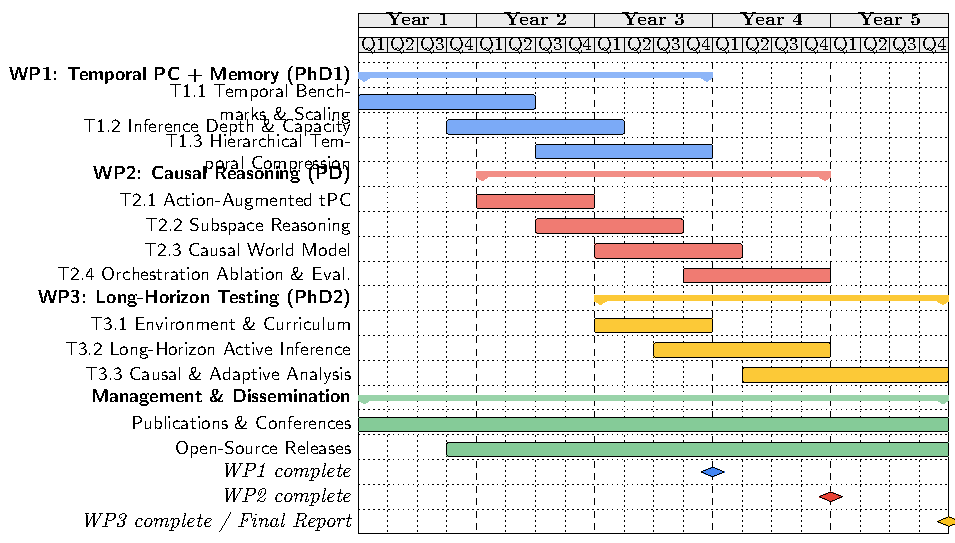
\includegraphics[width=\textwidth, clip]{figures/gantt-find.pdf}
    \caption{\textbf{FIND project Gantt chart (60 months).} WP1 (blue) Years 1--3, led by PhD1; WP2 (red) Years 2--4, led by PD; WP3 (yellow) Years 3--5, led by PhD2. Lepperød (PI, 50\%) provides scientific leadership across all WPs.}\label{fig:gantt}
\end{figure}


\noindent\textbf{Milestones:}
\begin{itemize}[noitemsep,topsep=2pt]
  \item \textbf{M1} (Month~12): PAM Tier~2 benchmarks complete; CORe50-NI results published.
  \item \textbf{M2} (Month~18): WP2 compositional reasoning prototype; extend PAMNCA with HDC composition.
  \item \textbf{M3} (Month~30): Memory Maze results at $T{=}10{,}000$.
  \item \textbf{M4} (Month~48): WP3 environment integration and agent evaluation.
  \item \textbf{M5} (Month~60): Final evaluation, open-source release, and benchmark suite.
\end{itemize}

\noindent\textbf{Estimated compute:} WP1: $\sim$20K GPU-hours; WP2: $\sim$30K GPU-hours (informed by PAMNCA's 15K hours for preliminary work); WP3: $\sim$50K GPU-hours. Total: $\sim$100K GPU-hours, covered by Simula eX3 and Sigma2 allocations.

\noindent\textbf{Team allocation:} Lepperød (PI, 50\%) provides scientific leadership across all WPs and leads WP2. The Postdoc (PD, 100\%) joins in Year~1 and co-leads WP2 with Lepperød, contributing to T2.1--T2.4. PhD1 (100\%) starts Year~1 and leads WP1 (T1.1--T1.3). PhD2 (100\%) starts Year~2 and leads WP3 (T3.1--T3.3). An additional PhD student may be hired in Year~3 depending on progress.

\subsection{Feasibility, risks, and contingency plans}

{\small
\noindent
\begin{tabularx}{\textwidth}{@{}p{1.3cm}Xp{0.8cm}p{0.8cm}X@{}}
\toprule
\textbf{Cat.} & \textbf{Description} & \textbf{Like.} & \textbf{Sev.} & \textbf{Mitigation} \\
\midrule
Scientific & Modular architecture fails to specialize. & Med & High & Progressive training with soft inductive biases; Gumbel-softmax entropy floor prevents module collapse. \\
 & Memory does not overcome catastrophic forgetting. & Med & High & Hybrid fast/slow memory with Bayesian consolidation; WTA write prevents slot mean-convergence. \\
 & tPC-KM fails to scale beyond MNIST. & Med & Med & Start with simplified environments; 4-tier benchmark hierarchy ensures incremental validation. \\
 & Compositional reasoning does not generalise beyond seen primitives. & Med & Med & Algebraic composition guarantees correctness by construction; FOMAML meta-learning for novel combinations. \\
Technical & Computational resources exceed expectations. & Med & Med & Sigma2 allocation + Simula eX3 cluster (${\sim}10^5$ GPU-hours); model distillation for efficiency. \\
 & Orchestration bottlenecks in information flow. & Med & High & Structured ablation ladder provides 4 fallback mechanisms ordered by complexity. \\
 & Active inference exploration is sample-inefficient. & Med & Med & Combine with imitation learning and adaptive curriculum; intrinsic motivation for efficient exploration. \\
Impl. & Environment integration (Minecraft/Factorio). & Med & Med & Simplified environment wrappers with fallback to Memory Maze; established Python APIs available. \\
Project & Recruitment of specialized expertise. & Med & Med & Leverage NORA network, ELLIS community, and international collaborations for candidate identification. \\
\bottomrule
\end{tabularx}
}

\noindent\textbf{Feasibility:} The preliminary results (98.1\% recall, $3.75{\times}$ less forgetting) demonstrate that the core architecture works. Each WP has independent value: even if WP3's most ambitious targets are not fully reached, WP1--2 produce publishable architectures and benchmarks. The structured ablation ladder in WP2 ensures that at least one orchestration mechanism will succeed. The 4-tier benchmark hierarchy provides natural checkpoints: if PAM does not surpass Tier~2, the Tier~3 targets are adjusted before investing in WP3 environments.

\subsection{Collaborations}

\noindent\textbf{Prof.\ Konrad Kording} (University of Pennsylvania): Bayesian decision theory and causal inference (WP2). One co-authored publication, ongoing collaboration since 2018. \textit{Tangible contribution:} Co-supervision of PD on causal world model formalism (T2.3); one PhD will visit Penn for 3 months in Year~3.

\noindent\textbf{Prof.\ Marc de Kamps} (University of Leeds): Computational neuroscience and compositional learning (WP2--3). Two co-authored publications, collaboration since 2016. \textit{Tangible contribution:} Collaboration on mean-field analysis of modular dynamics; joint workshops on biological plausibility of orchestration.

\noindent\textbf{Assoc.\ Prof.\ Blake Richards} (Mila/McGill): Normative models of hippocampal activity. Co-PI, PhD exchange program, ongoing since 2023. \textit{Tangible contribution:} PhD1 spends 6 months at Mila (Year~2) working on hippocampal models for WP1's hierarchical memory; joint publications on normative models of memory consolidation.

\noindent\textbf{Assoc.\ Prof.\ Arvind Kumar} (KTH): Neuromodulators in AI. Co-PI and co-author, ongoing since 2020. \textit{Tangible contribution:} Neuromodulatory gating mechanisms for memory consolidation (T1.3); joint supervision of PhD2.

\noindent\textbf{Prof.\ Stefan Leutgeb} (UC San Diego): Experimental spatial navigation. Visiting researcher 2017/2018, co-authored work submitted. \textit{Tangible contribution:} Experimental validation of PAM's spatial memory predictions against rodent place cell recordings.

\subsection{Integration into host institution}

Simula Research Laboratory is a Norwegian research institution with a strong track record in computational science. FIND will be hosted in the Department of Numerical Analysis and Scientific Computing (SCAN), within the BioAI group led by Lepperød. Simula provides:
\begin{itemize}[noitemsep,topsep=2pt]
  \item \textbf{Compute infrastructure:} Access to Simula's eX3 HPC cluster (A100/H100 GPUs) and national Sigma2 (Saga, Olivia) resources. WP3 RL experiments are estimated to require ${\sim}10^5$ GPU-hours (based on ${\sim}800$ GPU-hours per DreamerV3-scale training run $\times$ ${\sim}100$ experiments across curriculum stages and ablations). This exceeds Simula's internal allocation and motivates the additional equipment funding request.
  \item \textbf{Research environment:} Active AI research community, including the SURE-AI centre for industry collaboration, and connections to University of Oslo through Lepperød's adjunct professorship.
  \item \textbf{Training programs:} Simula Academy for researcher development; NORA Research School for PhD training; established supervision track record (2 PhDs completed, 4 in progress).
\end{itemize}

\subsection{Recruitment and ethics}

\noindent\textbf{Recruitment:} PhD and postdoc positions will be advertised internationally through NORA, ELLIS, and Simula's networks. We actively seek diverse candidates and will leverage our international collaborations for candidate identification. Simula's competitive salaries and Oslo's quality of life support strong recruitment.

\noindent\textbf{Ethics:} This research focuses on fundamental methods development in controlled game environments. No human subjects, animal data, or personal data are involved. We will follow Simula's Code of Ethics, the EU Ethics Guidelines for Trustworthy AI, and the EU AI Act. Beyond the project, applications of FIND technology would require evaluation of biases, security, and data governance.

\subsection*{Funding ID}

\begin{tabular}{p{3cm}p{3cm}p{6cm}p{2cm}}
\toprule
\textbf{Funder} & \textbf{Amount} & \textbf{Subject} & \textbf{Status} \\
\midrule
Simula internal & 4.5 MNOK/yr & BioAI group baseline funding & Active \\
RCN IKTPLUSS & 12 MNOK & PASSION: AI safety and alignment & Submitted \\
RCN FRIPRO & 10 MNOK & FIND (FRIPRO version): NeuroAI memory & Not funded \\
RCN IKTPLUSS & 12 MNOK & constrAIn: Constrained AI methods & Submitted \\
\bottomrule
\end{tabular}

\noindent The proposed ERC project is distinct from all listed funding. The FRIPRO FIND application (3-year, smaller scope) was not funded; the ERC proposal represents a substantially expanded 5-year programme with WP2 (compositional reasoning, validated by PAMNCA on ARC), WP3 (open-ended environments), the postdoc position, and substantial preliminary results (CORe50 continual learning, ARC program synthesis, HDC compositional reasoning benchmarks) not available at the FRIPRO submission.

\printbibliography[title={References}]

}

\end{refsection}

\end{document}
